\documentclass{exam}
\usepackage{units} 
\usepackage{graphicx}
\usepackage[fleqn]{amsmath}
\usepackage{cancel}
\usepackage{float}
\usepackage{mdwlist}
\usepackage{booktabs}
\usepackage{cancel}
\usepackage{polynom}
\usepackage{caption}
\usepackage{fullpage}
\usepackage{xfrac}
\usepackage{enumerate}

\newcommand{\degree}{\ensuremath{^\circ}} 
\everymath{\displaystyle}

\printanswers

% \begin{figure}[H]
%   \centering
%   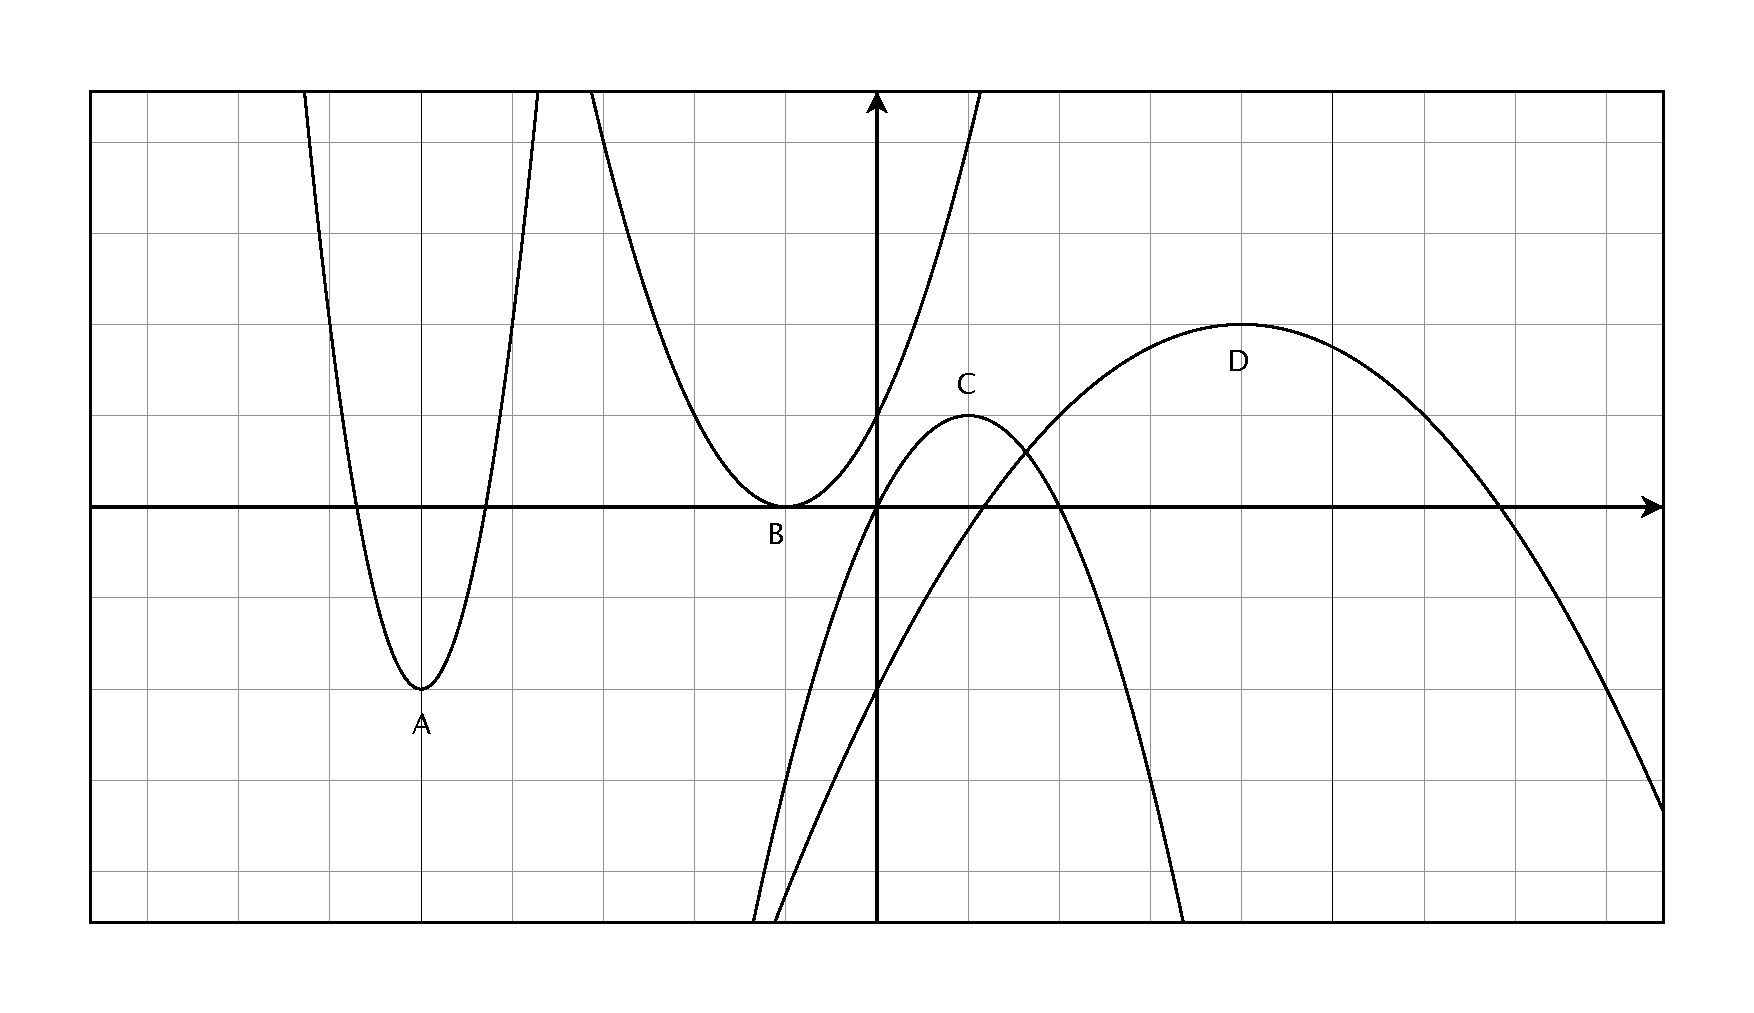
\includegraphics[scale=.3]{problem_7.eps}
%   \caption*{Problem 7}
% \end{figure}

% \begin{tabular}{cc}
% \toprule
% period & amplitude \\
% \midrule
%   $\pi$ & $2$ \\
% \bottomrule
% \end{tabular}

\title{Math 141 Notes \\ Section 3.3}
\date{April 10, 2013}

\begin{document}

  \maketitle
  \tableofcontents

  \pagebreak

  \section{Homework}
  \begin{itemize}
    \item When looking for candidates, sometimes you can make things easier by factoring out a constant.  See problem 6
      from homework 9.

    \item Talk to Jimmy about continuing from quotient instead of starting from original equation each time when looking
      for solutions.

    \item Don't forget to count the $x = 0$ solution (problem 63)

    \item Beau always one too many for total number of real zeros.
  \end{itemize}

  \section{Rational Zeros Theorem}

  \subsection{Description}
  For polynomials with integer coefficients, every rational zero is $\frac{p}{q}$, where $p$ is a factory of the constant
  coefficient and $q$ is a factor of the leading coefficient.

  \subsection{Proof}

  Find $f \left( \frac{p}{q} \right)$:
  \begin{align*}
    f(x)                         &= ax^3 + bx^2 + cx + d \\
    f \left( \frac{p}{q} \right) &= a \left( \frac{p}{q} \right)^3 + b \left( \frac{p}{q} \right)^2 + c \left( \frac{p}{q} \right) + d \\
  \end{align*}

  Set equal to zero and get rid of fractions:
  \begin{align*}
    a \left( \frac{p}{q} \right)^3 + b \left( \frac{p}{q} \right)^2 + c \left( \frac{p}{q} \right) + d &= 0 \\
    ap^3 + bp^2q + cpq^2 + dq^3                                                                        &= 0 \\
  \end{align*}

  Factor out $q$ to show $q$ is factor of $a$:
  \begin{align*}
    ap^3 + q(bp^2 + cpq + dq^2) &= 0 \\
    q(bp^2 + cpq + dq^2)        &= -ap^3 \\
  \end{align*}

  Factor out $p$ to show $p$ is factor of $d$:
  \begin{align*}
    p(ap^2 + bpq + cq^2) + dq^3 &= 0 \\
    p(ap^2 + bpq + cq^2)        &= -dq^3  \\
  \end{align*}

  % $q$ is a factor of $a_n$:
  % \begin{itemize*}
  %   \item $\frac{p}{q}$ is a rational zero
  %   \item plug $\frac{p}{q}$ in to polynomial
  %   \item multiply by $q^n$
  %   \item factor out $p$ to get $p(\ldots) = -a_0 q^n$.  $p$ is a factor of left side so it must be factor of right side.
  %     $p$ is not a factor of $q$ so it must be a factor of $a_0$.
  %   \item factor out $q$ to get $q(\ldots) = -a_0 p^n$.  $q$ is a factor of left side so it must be factor of right side.
  %     $q$ is not a factor of $p$ so it must be a factor of $a_n$.
  % \end{itemize*}

  \subsection{Procedure}
  \begin{itemize*}
    \item list possible zeros
    \item divide
    \item repeat
  \end{itemize*}

  \subsection{Examples}
  \begin{enumerate}

    \item
      \begin{align*}
        P(x) &= x^3 - 7x - 6 \\
             &= (x + 1)(x - 3)(x + 2) \\
        \\
        x    &= \left\{ 1, 2, 3, 6 \right\} \\
      \end{align*}

    \item 
      \begin{align*}
        P(x) &= x^3 + 4x^2 - 7x - 10 \\
             &= (x + 5) (x - 2) (x + 1) \\
        \\
        x    &= \left\{ 1, 2, 5, 10 \right\} \\
      \end{align*}

    \item 
      \begin{align*}
        P(x) &=x^3 + 3x^2 - 4x - 12 \\
             &= (x - 2) (x + 3) (x + 2) \\
        \\
        x    &= \left\{ 1, 2, 3, 4, 6, 12 \right\} \\
      \end{align*}

    \item 
      \begin{align*}
        P(x) &= 2x^3 + 5x^2 - 4x - 3 \\
             &= (2x + 1) (x - 1) (x + 3) \\
        \\
        x    &= \left\{ \frac{1}{2}, 1, \frac{3}{2}, 3 \right\} \\
      \end{align*}

    \item 
      \begin{align*}
        P(x) &= 3x^3 + 5x^2 - 4x - 4 \\
             &= (3x + 2) (x - 1) (x + 2) \\
        \\
        x    &= \left\{ \frac{1}{3}, \frac{2}{3}, 1, \frac{4}{3}, 2, 4 \right\} \\
      \end{align*}

    \item 
      \begin{align*}
        P(x) &= 2x^3 - 3x^2 - 11x + 6 \\
             &= (x-3) (x+2) (2x-1) \\
        \\
        x    &= \left\{ \frac{1}{2}, 1, \frac{3}{2}, 2, 3, 6 \right\} \\
      \end{align*}

    \item 
      \begin{align*}
        P(x) &= 2x^3 - 5x^2 - 14x + 8 \\
             &= (x - 4) (x + 2) (2x - 1) \\
        \\
        x    &= \left\{ \frac{1}{2}, 1, 2, 4, 8 \right\} \\
      \end{align*}

  \end{enumerate}

  Use quadratic formula to find last few zeros:
  \begin{enumerate}
    \item 
      \begin{align*}
        P(x)    &= x^3 - 6x + 4 \\
                &= (x - 2) (x^2 + 2x - 2) \\
        x       &= \left\{ 1, -1 \pm \sqrt{3} \right\} \\
        \\
        x       &= \left\{ 1, 2, 4 \right\} \\
      \end{align*}

    \item 
      \begin{align*}
        P(x)    &= x^3 + 2x^2 - 4x + 1 \\
                &= (x - 1) (x^2 + 3 x - 1) \\
        x       &= \left\{ 1, \frac{-3 \pm \sqrt{13}}{2} \right\} \\
        \\
        x       &= \left\{ 1, 2, 4 \right\} \\
      \end{align*}
  \end{enumerate}

  \section{Descartes' Rule of Signs}

  \subsection{Description}
  \begin{itemize}
    \item The number of positive real zeros of $P(x)$ is equal to the number of variations in sign in $P(x)$ or less than that
      by an even whole number.

    \item The number of negative real zeros of a polynomial is equal to the number of variations in sign in $P(-x)$ or
      less than that by an even whole number.

    \item Variations in sign is positive to negative or vice versa, skipping zeros

    \item Use to rule out additional possibilities after finding some of the zeros
  \end{itemize}

  \subsection{Examples}

  \begin{enumerate}
    \item 
      \begin{align*}
        P(x)    &= x^3-3 x^2-6 x+8 \\
                &= (x - 1) (x + 2) (x - 4) \\
        \\
        x       &= \left\{ 1, 2, 4, 8 \right\} \\
      \end{align*}

      \begin{itemize*}
        \item 2 or 0 positive roots
        \item 1 negative root
      \end{itemize*}

    \item 
      \begin{align*}
        P(x)    &= x^3-9 x^2+23 x-15 \\
                &= (x - 5) (x - 1) (x - 3) \\
        \\
        x       &= \left\{ 1, 3, 5, 15 \right\} \\
      \end{align*}

      \begin{itemize*}
        \item 3 or 1 positive roots
        \item 0 negative roots
      \end{itemize*}

  \end{enumerate}

  \section{Upper and Lower Bounds Theorem}

  \subsection{Description}

  \begin{itemize}
    \item If we divide $P(x)$ by $x - b$ with $b > 0$ and the row that contains the answer has no negative entry, then
      $b$ is an upper bound for the real zeros of $P$.

    \item If we divide $P(x)$ by $x - a$ with $a < 0$ and the row that contains the answer has alternate non-positive and
      non-negative, then $a$ is a lower bound for the real zeros of $P$.

  \end{itemize}

  \begin{align*}
    P(x)    &= 2 x^3 - 3 x^2 - 8 x + 12 \\
            &= (x-2) (x+2) (2 x-3) \\
    \\
    x       &= \left\{ \frac{1}{2},1,\frac{3}{2},2,3,4,6,12 \right\} \\
  \end{align*}

  3 is an upper bound:
  \[ \polyhornerscheme[x = 3]{2 x^3 - 3 x^2 - 8 x + 12} \]

  -3 is a lower bound
  \[ \polyhornerscheme[x = -3]{2 x^3 - 3 x^2 - 8 x + 12} \]

  \subsection{Proof}

  \subsubsection{Part One}
  \begin{itemize*}
    \item Dividing $P(x)$ by $(x - b)$ gives some quotient polynomial $Q(x)$ and a remainder: 
      \[
        P(x) = (x - b)Q(x) + r
      \]

    \item Evaluate at any number $c$ where $c > b$:
      \[
        P(c) = (c - b)Q(c) + r
      \]

    \item If all the coefficients in $Q$ are non-negative and $c > b$:
      \begin{enumerate*}
        \item Since $c > b$, $c - b > 0$
        \item $Q(c) > 0$ since all the coefficients are positive and $c$ is positive
        \item $r \geq 0$, since the final row contained only non-negative values
      \end{enumerate*}

      Therefore $P(c) > 0$ and $c$ is not a root of $P$.

  \end{itemize*}

  \subsubsection{Part Two}

  One approach is to realize that if $x$ is solution to $f(x)$, $-x$ is a solution to $f(-x)$, etc.

  Another approach is:
  \begin{itemize*}
    \item if $f(x) = a_nx^n - a_{n-1}x^{n-1} + a_{n-2}x^{n-2} \ldots$ alternates signs, then $f(-x)$ has all the same sign
      because all the odd powers change sign.

    \item If all the terms are negative, $f(a)$ is negative and any value less than $a$ will only result in a more
      negative value, not zero.

    \item If all the terms are positive, $f(a)$ is positive and any value less than $a$ will only result in a more
      positive value, not zero.

%    \item if $-b$ is an upper bound to the solutions for $f(-x)$, $b$ is a lower bound for the solutions of $f(x)$
%      (reflection around y-axis).  
%
%    \item Suppose $b$ satisfies the second part for $f(x)$ ($b < 0$ and alternating signs).  Then $-b$ satisfies first part
%      ($b > 0$ and all same sign.  $-b$ is an upper bound for $f(-x)$, so $b$ is a lower bound for $f(x)$.

  \end{itemize*}

  \subsection{Examples}

  \begin{enumerate}
    \item 
      \begin{align*}
        P(x)    &= 2x^3 - 3x^2 - 8x + 12 \\
                &= (x - 2)(x + 2)(2x - 3) \\
        \\
        x       &= \left\{ \frac{1}{2},1,\frac{3}{2},2,3,4,6,12 \right\} \\
      \end{align*}

      3 is an upper bound:
      \[ \polyhornerscheme[x = 3]{2x^3 - 3x^2 - 8x + 12} \]

      -3 is a lower bound
      \[ \polyhornerscheme[x = -3]{2x^3 - 3x^2 - 8x + 12} \]

    \item 
      \begin{align*}
        P(x)    &= x^3 - 5x^2 - 2x + 24 \\
                &= (x - 3)(x + 2)(x - 4) \\
        \\
        x       &= \left\{ \frac{1}{2},1,\frac{3}{2},2,3,4,6,12 \right\} \\
      \end{align*}

      6 is an upper bound:
      \[ \polyhornerscheme[x = 6]{x^3 - 5x^2 - 2x + 24} \]

      -3 is a lower bound
      \[ \polyhornerscheme[x = -3]{x^3 - 5x^2 - 2x + 24} \]

  \end{enumerate}

\end{document}
